\documentclass[assignment4.tex]{subfiles}
\begin{document}

\section*{2η Άσκηση}
Το πρόβλημα ρίψης σφαίρας από το έδαφος με αρχική ταχύτητα, λαμβάνοντας υπόψιν μόνο την δύναμη της βαρύτητας, μπορεί να διατυπωθεί μαθηματικά εφαρμόζοντας το δεύτερο νόμο του \textlatin{Newton}, από τον οποίον προκύπτει το σύστημα διαφορικών εξισώσεων με αρχικές συνθήκες (\ref{eq:newton_equations}).
\begin{equation}
\left\{
	\begin{matrix}
	m\frac{d^2x}{dt^2} =& 0 \\
	m\frac{d^2y}{dt^2} =& -mg \\
	x(0) =& 0 \\
	y(0) =& 0 \\
	x'(0) =& v_0 \cos \frac{\pi}{4} \\
	y'(0) =& v_0 \sin \frac{\pi}{4}
	\end{matrix}
\right.
\label{eq:newton_equations}
\end{equation}

Για να λυθεί το σύστημα με αριθμητικές μεθόδους, πρέπει να έρθει σε κατάλληλη μορφή $u'=f(t,u)$, όπου $u$ διάνυσμα με άγνωστες συναρτήσεις, $t$ η ανεξάρτητη μεταβλητή και $f$ κατάλληλη συνάρτηση. Ορίζεται $u_0=x$, $u_1=x'$, $u_2=y$ και $u_3=y'$, οπότε οι εξισώσεις (\ref{eq:newton_equations}) μετασχηματίζονται σε μορφή πινάκων (\ref{eq:newton_equations_matrix})
\begin{equation}
\underbrace{\frac{d}{dt}\left[
\begin{matrix}
u_0 \\
u_1 \\
u_2 \\
u_3
\end{matrix}
\right]
}_{u'}
=
\underbrace{\left[
\begin{matrix}
0 & 1 & 0 & 0\\
0 & 0 & 0 & 0\\
0 & 0 & 0 & 1\\
0 & 0 & 0 & 0
\end{matrix}
\right]
}_{A}
\underbrace{\left[
\begin{matrix}
u_0 \\
u_1 \\
u_2 \\
u_3
\end{matrix}
\right]
}_{u}
+
\underbrace{\left[
\begin{matrix}
0 \\
0 \\
0 \\
-g
\end{matrix}
\right]
}_{b}
,
\underbrace{\left[
	\begin{matrix}
	0 \\
	v_0\cos\frac{\pi}{4} \\
	0 \\
	v_0 \sin\frac{\pi}{4}
	\end{matrix}
	\right]
}_{u(0)}
\label{eq:newton_equations_matrix}
\end{equation}
ή συνοπτικά (\ref{eq:newton_equations_symb}), όπου αντιστοιχεί $f(t, u)=Au + b$. Σε αυτή τη μορφή το σύστημα διαφορικών εξισώσεων είναι επιλύσιμο με το σχήμα \textlatin{Euler} ή \textlatin{Runge-Kutta} 4ης τάξης.
\begin{equation}
u' = Au + b, u_0=u(0)
\label{eq:newton_equations_symb}
\end{equation}
Συγκεκριμένα, για το σχήμα \textlatin{Euler}, εφαρμόζεται η υπολογιστική διαδικασία (\ref{eq:euler_scheme}),
\begin{equation}
u_{i+1} = u_i + hf(t_i, u_i) , u_0=u(0)
\label{eq:euler_scheme}
\end{equation}
ενώ στο σχήμα \textlatin{Runge-Kutta} η (\ref{eq:rungekutta_scheme}).
\begin{equation}
\begin{split}
k_1 =& f(t_i, u_i) \\
k_2 =& f(t_i+\frac{h}{2}, u_i+\frac{h}{2}k_1) \\
k_2 =& f(t_i+\frac{h}{2}, u_i+\frac{h}{2}k_2) \\
k_3 =& f(t_i+h, u_i + h k_3) \\
u_{i+1} =& u_i + \frac{h}{6}\left(k_1 + 2k_2 + 2k_3+ k_4\right), u_0=u(0)
\end{split}
\label{eq:rungekutta_scheme}
\end{equation}

Η επίλυση του συστήματος διαφορικών εξισώσεων με τη μέθοδο \textlatin{Euler} για διάφορα μεγέθη χρονικού βήματος παράγει τα Σχήματα \ref{fig:ex2Euler_x} και \ref{fig:ex2Euler_y}. Μαζί με την αριθμητική λύση δίνεται και η αναλυτική που δίνεται από τις εξισώσεις \ref{eq:analytic}.
\begin{equation}
\left\{
\begin{matrix}
x(t) =& v_0\cos(\phi) t \\
y(t) =& v_0\sin(\phi) t - \frac{1}{2}gt^2
\end{matrix}
\right.
\label{eq:analytic}
\end{equation}
Η σύγκριση αποκαλύπτει ότι η αριθμητική λύση της $x(t)$ συμπίπτει με την αναλυτική για κάθε μέγεθος βήματος, που είναι αναμενόμενο γιατί η λύση είναι γραμμική συνάρτηση και συμπίπτει με την προσέγγιση πρώτης τάξης της μεθόδου \textlatin{Euler}. Ωστόσο, για την $y(t)$ που είναι πολυώνυμο 2ου βαθμού, απαιτείται αρκετά μικρό βήμα $h<0.01$ προκειμένου να προσεγγιστεί ικανοποιητικά η αναλυτική. Μικρότερο βήμα συνεπάγεται μεγαλύτερο αριθμό βημάτων, δηλαδή 142 (και 283 για $h=0.005$). 
\begin{figure}[hp]
	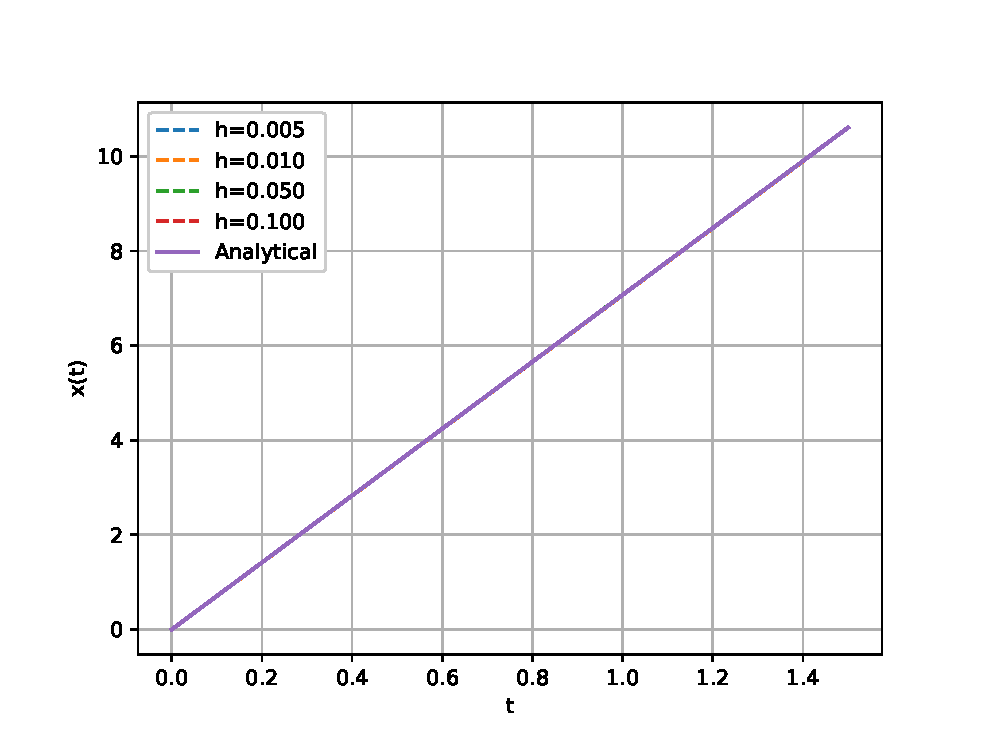
\includegraphics[width=0.9\textwidth]{ex2Euler_x.eps}
	\centering
	\caption{Μέθοδος \textlatin{Euler} - $x(t)$}
	\label{fig:ex2Euler_x}
	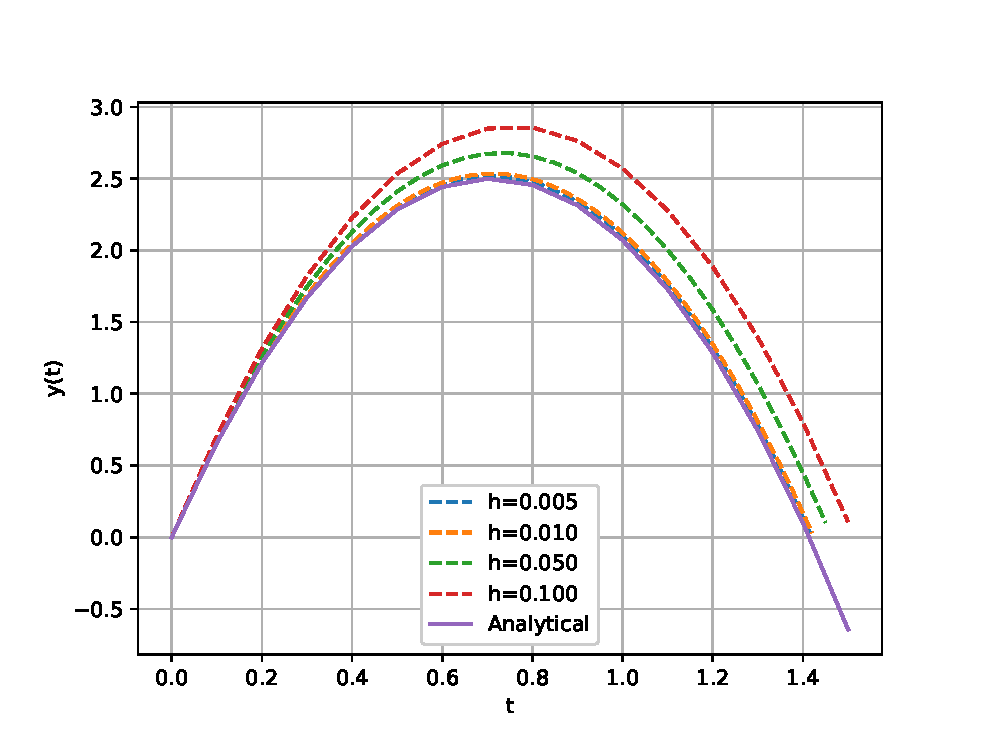
\includegraphics[width=0.9\textwidth]{ex2Euler_y.eps}
	\centering
	\caption{Μέθοδος \textlatin{Euler} - $y(t)$}
	\label{fig:ex2Euler_y}
\end{figure}

Η εφαρμογή της μεθόδου \textlatin{Runge-Kutta} 4ης τάξης, παράγει καλύτερα αποτελέσματα. Και πάλι η αριθμητική λύση της $x(t)$ συμπίπτει με την αναλυτική, αλλά επιπλέον η αριθμητική λύση της $y(t)$ είναι πολύ κοντά στην αναλυτική ακόμα και για $h=0.1$, δηλαδή μεγαλύτερο κατά μία τάξη μεγέθους σε σχέση με την \textlatin{Euler}. Τα αποτελέσματα δίνονται στα Σχήματα \ref{fig:ex2RungeKutta_x} και \ref{fig:ex2RungeKutta_y}. O αριθμός των βημάτων για κάθε μέγεθος βήματος είναι ίδιος, αλλά εφόσον η \textlatin{Runge-Kutta} αποκλίνει πολύ λίγο από τη αναλυτική λύση για μεγάλο βήμα, αποδεικνύεται και η υπεροχή της ως προς την \textlatin{Euler}.

\begin{figure}[hp]
	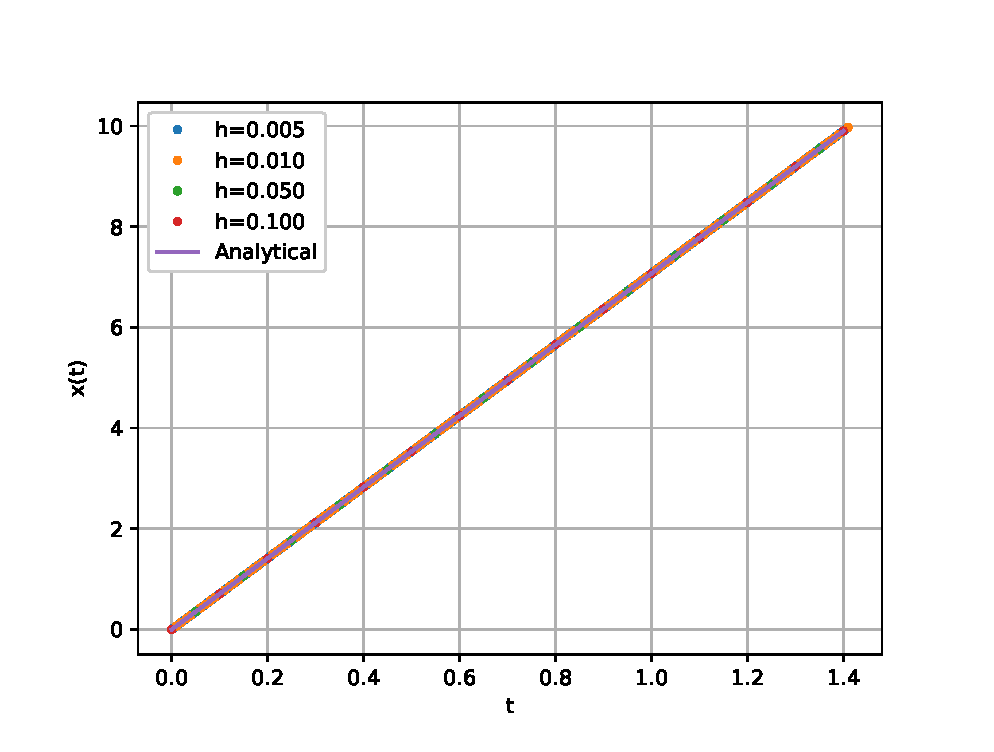
\includegraphics[width=0.9\textwidth]{ex2RungeKutta_x.eps}
	\centering
	\caption{Mέθοδος \textlatin{Runge-Kutta} 4ης - $x(t)$}
	\label{fig:ex2RungeKutta_x}
	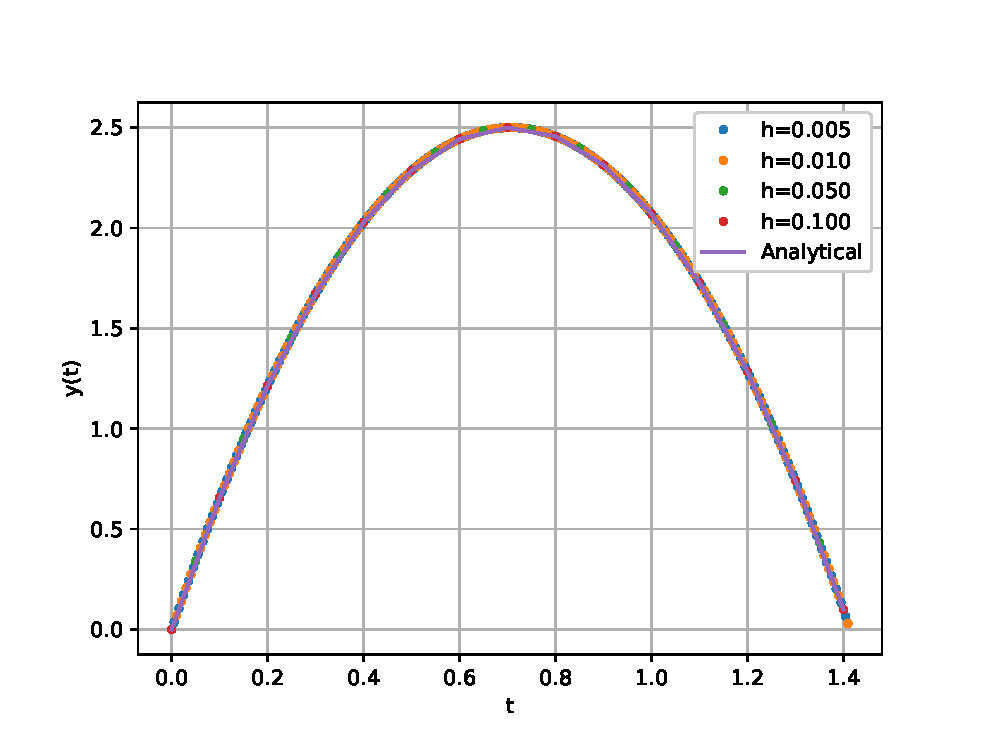
\includegraphics[width=0.9\textwidth]{ex2RungeKutta_y.eps}
	\centering
	\caption{Mέθοδος \textlatin{Runge-Kutta} 4ης - $y(t)$}
	\label{fig:ex2RungeKutta_y}
\end{figure}

Παρακάτω ακολουθεί ο κώδικας που γράφτηκε σε \textlatin{Python} και έγινε χρήση της βιβλιοθήκης \textlatin{Numpy}. Οι αλγόριθμοι \textlatin{Euler} και \textlatin{Runge-Kutta} 4ης τάξης δίνονται στο Παράρτημα.
\selectlanguage{english}
\lstinputlisting[style=python, firstline=8]{ex2.py}
\end{document}